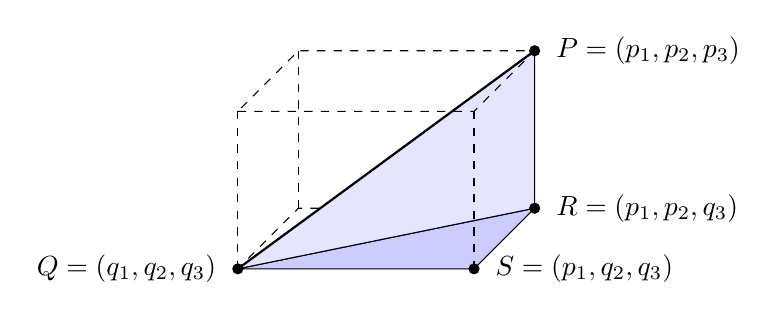
\begin{tikzpicture}[scale=1]
    \draw[dashed] (3,0,-2) -- (0,0,-2) -- (0,0,0);
    \draw[dashed] (0,0,0) -- (0,2,0);
    \draw[dashed] (0,0,-2) -- (0,2,-2);
    \draw[fill=blue!20] (0,0,0) -- (3,0,0) -- (3,0,-2) -- cycle;
    \draw[fill=blue!10] (0,0,0) -- (3,0,-2) -- (3,2,-2) -- cycle;
    \draw[dashed] (0,2,0) -- (3,2,0) -- (3,2,-2) -- (0,2,-2) -- cycle;
    \draw[dashed] (3,0,0) -- (3,2,0);
    \draw[thick] (0,0,0) -- (3,2,-2);
    \draw[fill](0,0,0) circle [radius=1.8pt] node[left=1ex]{$Q=(q_1,q_2,q_3)$};
    \draw[fill](3,2,-2) circle [radius=1.8pt] node[right=1ex]{$P=(p_1,p_2,p_3)$};
    \draw[fill](3,0,-2) circle [radius=1.8pt] node[right=1ex]{$R=(p_1,p_2,q_3)$};
    \draw[fill](3,0,0) circle [radius=1.8pt] node[right=1ex]{$S=(p_1,q_2,q_3)$};
  \end{tikzpicture}
